\chapter{Datarらのアルゴリズム}

本章では,Datarら \cite{Datar} によって提案されたデータストリームに対するハッシュ値更新アルゴリズムを
記述する.本論文での提案手法は,このアルゴリズムを基に多重集合へ拡張したものである.
データストリームとは,毎時刻要素$e$が到着するデータである.
Datarらの手法はデータストリームのスライディングウィンドウモデルに従って集合が変化することを仮定している.

\section{スライディングウインドウモデル}
時刻$t$における集合を$A_t=\{e_{t-w+1},e_{t-w+2},\cdots,e_t\}$とする.$w$はスライディングウインドウの幅であり,
$A_t$は$w$個の要素で構成される.また,$A_t$の要素は到着時間順に並んでいる.図\ref{fig:window}では,$w=4$の時
に3つの時刻$t$,$t+1$,$t+2$に対する集合$A_t,A_{t+1},A_{t+2}$を図示している.そして,時刻によってスライディングウインドウは変化していく.
例えば,図\ref{fig:window}のようにデータストリーム$\{a,f,h,e,k,q,o,g\}$となっていて,ウインドウサイズ$w=4$とすると,時刻$t$では,
$A_{t}=\{e_{t-3},e_{t-2},e_{t-1},e_t\}$であり,時刻$t +1$では,$A_{t+1}=\{e_{t-2},e_{t-1},e_t,e_{t+1}\}$となる.

\begin{figure}[H]
 \centering
 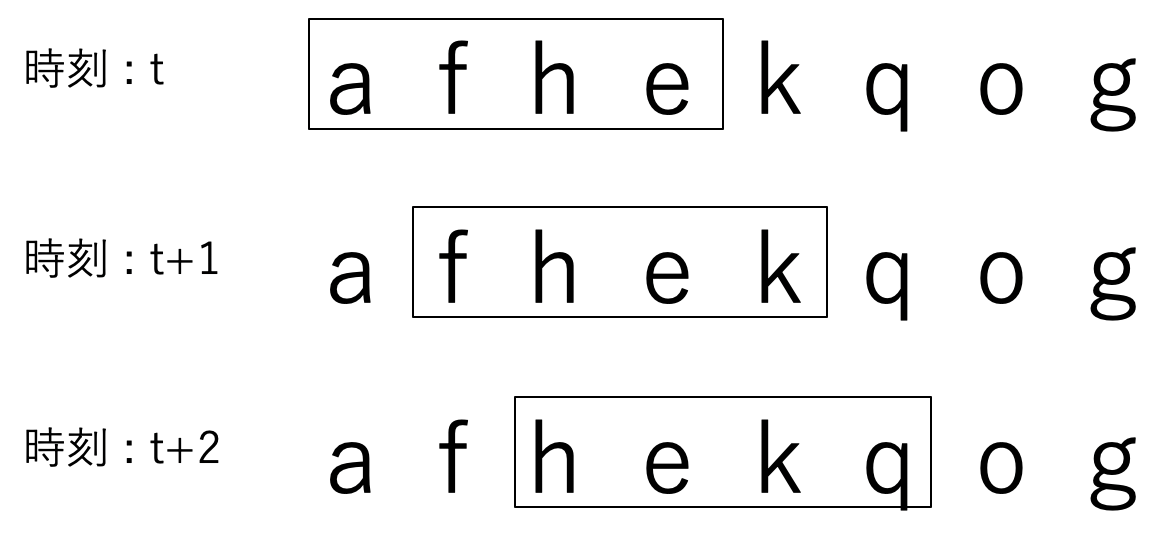
\includegraphics[width=15cm]{3_2_Ver1.1.png}
 \caption{スライディングウインドウ}
\label{fig:window}
\end{figure}

動的に変化する集合に対してハッシュ値を計算する自明な手法は,時刻経過によりウインドウがスライドするたびにハッシュ値を完全に
再計算するやり方である.これはすなわち,時刻が$t$から$t+1$に変化した際に,$h(A_{t+1})$を$A_{t}$とは無関係に計算するということ
である.この手法では,毎時刻ウィンドウ内の全要素をスキャンする必要があるので,$h(A_{t+1})$を求めるための時間計算量は$O(w)$
となる.

しかし、$A_t$と$A_{t+1}$は$e_t$と$e_{t+w}$以外の$w-1$個の要素が共通であり,$h(A_t)$計算時に判明した情報を再利用すること
で$h(A_{t+1})$を計算するオーバーヘッドを減らせる可能性がある.

\section{Datarらの手法}
Datar[1]らの手法の基本アイデアは
\begin{itemize}
\item 将来に割り当て値が最小になる可能性が絶対にない要素をあらかじめ削除することで,
次の時刻のハッシュ値$h(A_{t+1})$を計算する時に参照する要素数を減らす
\end{itemize}
というものである.ここで割り当て値が最小になる可能性が絶対にない要素とは,「ウィンドウ内で自分より後方に割り当て値が小さい要素が存在
する要素」のことである.例えば,$A_{t}$内の2要素$e_i$と$e_j$ ($i<j$)の割り当て値が$\pi(e_i)>\pi(e_j)$を満たすとしよう.
この時,$e_i$は自分より後方に割り当て値が小さい$e_j$が存在するという条件を満足する.この条件の下では$e_i$がウィンドウ内に存在する期間は$e_j$も必ずスライディングウィンドウ内に存在するので,$e_i$の割り当て値が最小になることはありえない(図\ref{fig:datar_ML} ).
Datarの手法ではこの性質を利用して,スライディングウインドウから最小値になりえない要素を削除し,将来最小値になりうる要素のみをMinlistというリストで管理する.
%Datarの手法ではこの性質を利用して,スライディングウインドウ内で将来最小値になりうる要素のリストMinlistを作成して管理する.
$A_t$のハッシュ値はMinlistに残った要素の割り当て値の最小値となる.
%\begin{equation}
 %\label{eq:datar}
%h(A_t)= \min_{e \in \mbox{Minlist}} \pi(e).
%\end{equation}
任意のMinlist内の要素$e$に対して,$e$より後方に割り当て値$\pi(e)$より小さい要素は存在しないので,
Minlist内の要素群に対する割り当て値は単調増加となる.このため,$h(A_{t})$は実はMinlistの先頭要素の
割り当て値と等しい.

\begin{figure}[H]
 \centering
 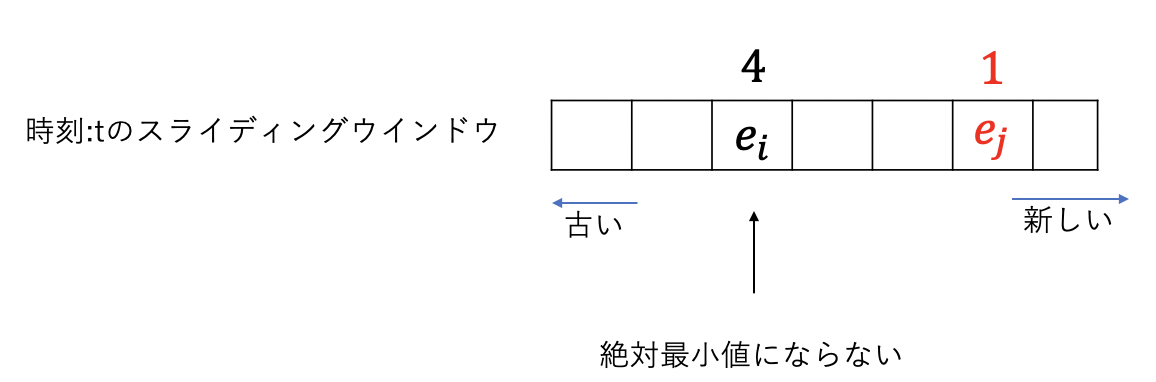
\includegraphics[width=15cm]{datar_ML.png}
 \caption{スライディングウインドウモデルの性質}
 \label{fig:datar_ML}
\end{figure}

時刻が$t$から$t+1$に変化した時にMinlistを更新する手順を以下にまとめる.
\begin{itemize}
\item $e_{t-w+1}$がウィンドウから離脱した時の処理\\
$e_{t-w+1}$がMinlistに含まれる時には$e_{t-w+1}$をMinlistから削除する.この時,$h(A_t)=\pi(e_{t-w+1})$であるため,ハッシュ値を更新する必要がある.そのため,$h(A_{t+1})$を新たにMinlistの先頭になった要素の割り当て値とする.
\item $e_{t+1}$をウィンドウに追加した時の処理\\
Minlist内で割り当て値が$\pi(e_{t+1})$より大きい要素は,今後,割り当て値が最小になりえないので削除する.
$e_{t+1}$によりMinlist内の他の要素がすべて削除された結果,Minlistに$e_{t+1}$のみ残った場合は
$h(A_{t+1})=\pi({e_{t+1}})$とする.
\end{itemize}


このアルゴリズムの動きを図 \ref{fig:koho2} に例示する.

%一番最初にスライディングウインドウからMinlistを作成する時は,前の要素から一つずつ見ていって,候補リストに加えていく.その過程で,加えた要素より前に自分より大きい要素があれば削除する.その工程を一番後ろの要素まで行うと単調増加の候補リストが作成される.これは候補リストの中で一番前の要素が一番小さく,Min-hashによるハッシュ値の値となるということである.そして,

時刻t+1の時,スライディングウインドウから一番前の要素$e_{t-w+1}$を削除し,新しい要素$e_t+1$のアルファベットkが入ってくる.kの割り当て値は3であるので,Minlistの中から3より大きい割り当て値を持つ要素を削除し,候補リストの一番後ろにkの割り当て値3を加える.
%つまり,スライディングウインドウ更新の際は,一番古い要素が候補リストに入って入れば削除し,新しい要素の割り当て値より大きい値が候補リストに存在する場合は,その中から削除する.そして,候補リストの一番後ろに新しい要素の割り当て値を加える.


\begin{figure}[H]
 \centering
 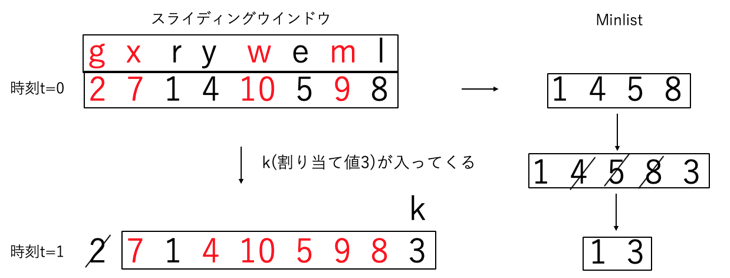
\includegraphics[width=15cm]{koho2.png}
 \caption{候補リストの作成}
 \label{fig:koho2}
\end{figure}

このようにDatarらは作成した最小値の候補リストを持ちいることにより,スライディングウインドウを保持する必要がない.そのため,ウインドウサイズWの場合, 候補リストは$\log(W)$で保持することができ,二部探索で候補リストを探索し,実行時間は$\log\log(W)$となることが保証される.
